\subsection{Consistency Check}

We need to check the consistency between main/sub traces to ensure that the trace data is consistent.

\subsubsection{Consistency between Main Trace and Sub Traces}

According to the definition of main/sub trace tables, elements of sub trace tables should be taken from the main trace table. For example, the RAM sub trace table is composed of all RAM operations in main trace table, the signature sub trace table is composed of all signature verification operations in the main trace table. Now we need to make sure that these are executed correctly. Lookup Argument gracefully achieves this through successfully binding the data relationship between the main trace table and the corresponding sub trace tables.

\begin{figure}[!ht]
    \centering
    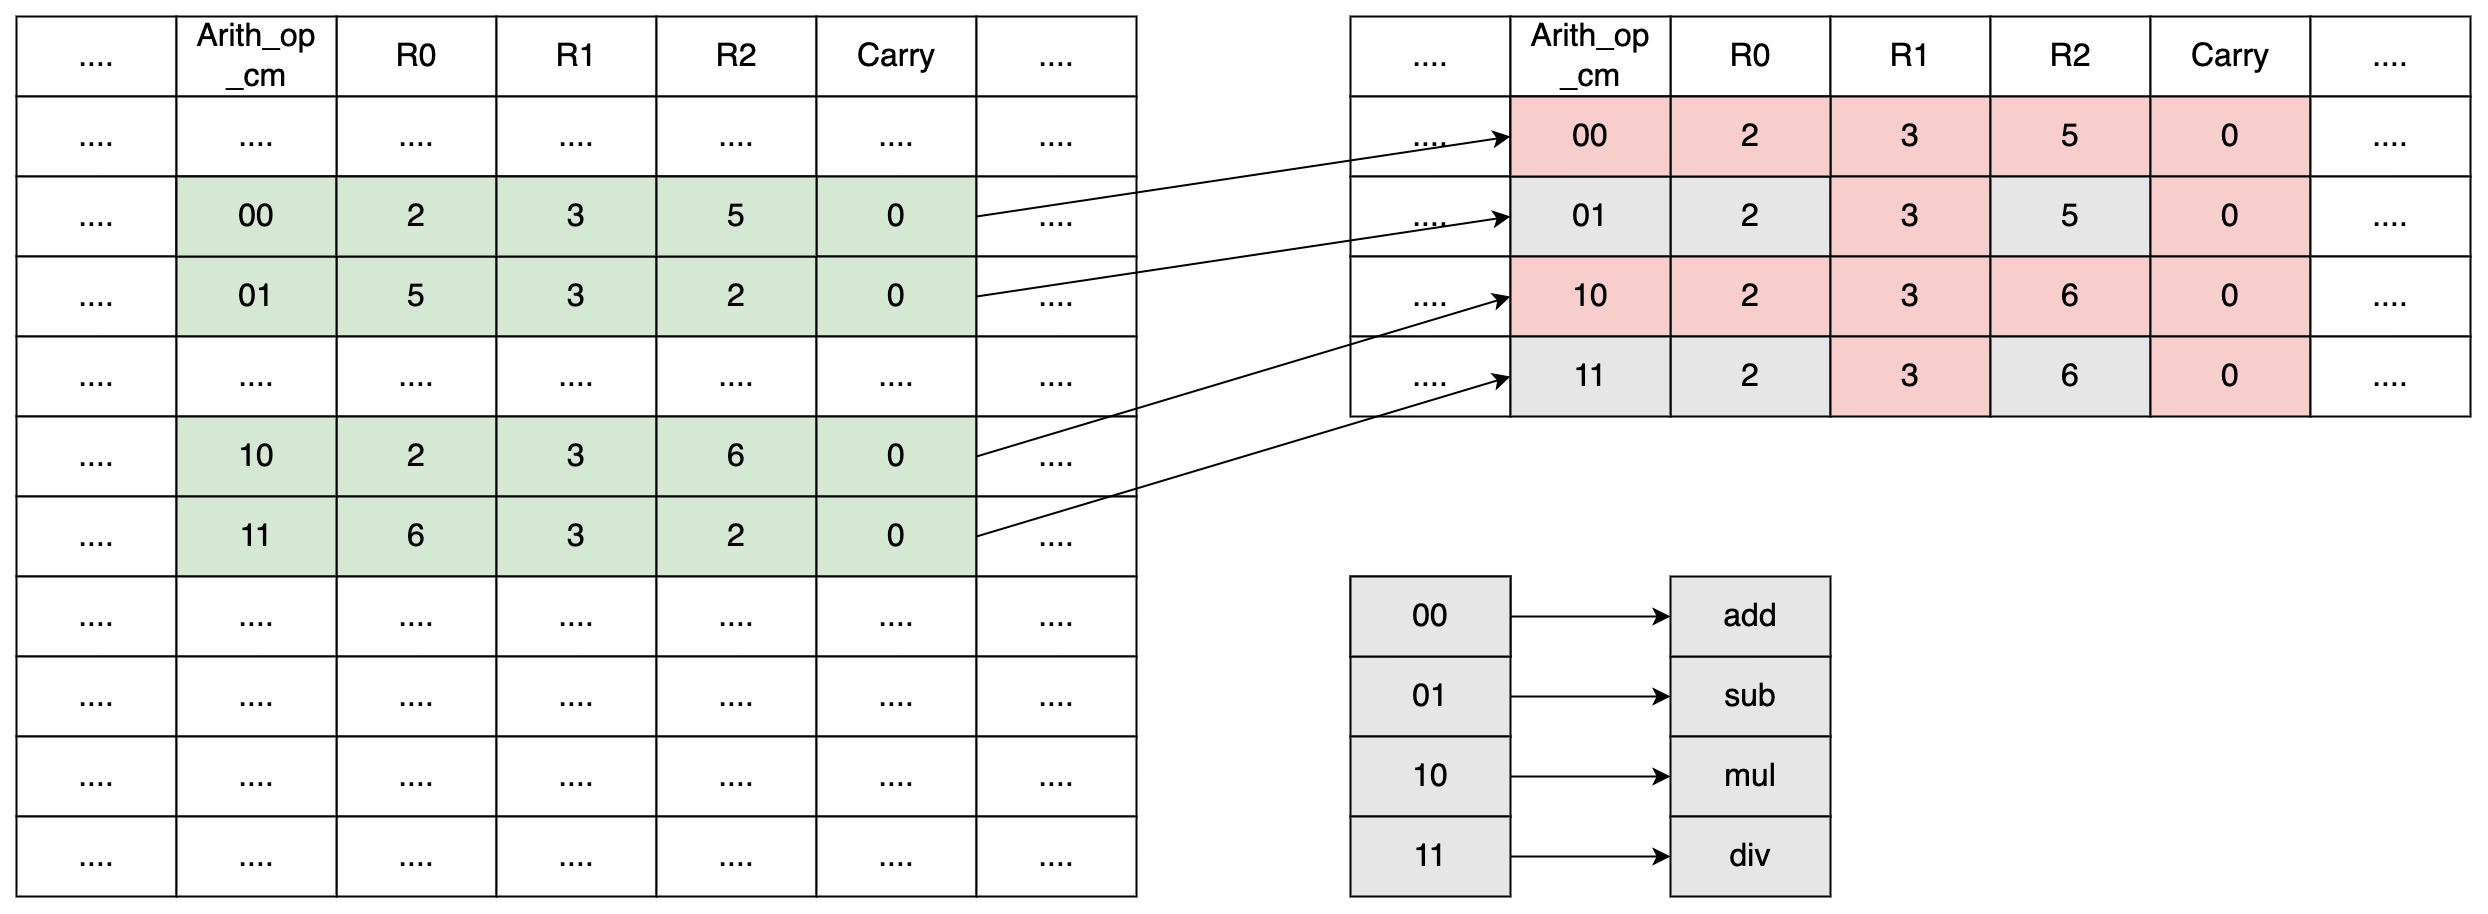
\includegraphics[width=0.8\textwidth]{main-sub-trace-lookup.jpg}
    \caption{Lookup between main trace and sub trace tables}
    \label{fig:main-sub-trace-lookup}
\end{figure}

\emph{Note:} We have adjusted subtraction and division for convenience (The gray marked part on the right side of Figure \ref{fig:main-sub-trace-lookup}), so that addition and subtraction can share one set of constraints and multiplication and division can share another set of constraints, which minimizes the overall constraints scale.

We utilize Lookup technology to ensure data consistency between the main trace table on the left and sub trace tables on the right, such as
\[ \{\text{arith\_op\_cm}, \text{R0}, \text{R1}, \text{R2}, \text{Carry}\}_\text{sub trace table} \subset \{\text{arith\_op\_cm}, \text{R0}, \text{R1}, \text{R2}, \text{Carry}\}_\text{main trace table} \]

Utilizing the following constraints to verify the validity of the data in sub trace tables
\begin{align*}
    f_{\text{arith\_op\_cm}}(x) \prod \left(3 - f_{\text{arith\_op\_cm}}(x)\right) \left(4 - f_{\text{arith\_op\_cm}}(x)\right) \left(f_{\text{R0}}(x) + f_{\text{R1}}(x) - (f_{\text{R2}}(x) + \mathrm{Bound} \cdot f_{\text{Carry}}(x))\right) &= 0, \\
    f_{\text{arith\_op\_cm}}(x) \prod \left(1 - f_{\text{arith\_op\_cm}}(x)\right) \left(2 - f_{\text{arith\_op\_cm}}(x)\right) \left(f_{\text{R0}}(x) \cdot f_{\text{R1}}(x) - (f_{\text{R2}}(x) + \mathrm{Bound} \cdot f_{\text{Carry}}(x))\right) &= 0.
\end{align*}

\emph{Note:} The idea of Combined Selector is adopted here to reduce the number of selector polynomials. Please refer to Section \ref{sec:key-technologies} for detailed principles.

\subsubsection{Consistency between Sub Traces}

As mentioned in the previous section, we ensure data consistency between the main/sub trace tables through Lookup Arguments, however, data consistency must also be maintained between sub trace tables. For example, we store the result of instruction \verb|ADD| in a result register, we must be able to ensure that the value written in this register is indeed the result of the execution of that previous instruction. Then we utilize Permutation Arguments to ensure data consistency between the arithmetic sub trace table and the RAM sub trace table.

During the execution of the entire VM, some of the operands of the instructions derive from intermediate values of the VM execution, when utilizing Permutation Argument to ensure data consistency as mentioned above, some derive from public inputs, such as the initial value and result of the program, we use instruction \verb|EQ| to ensure that the instruction does operate the correct value.
\begin{figure}[!ht]
    \centering
    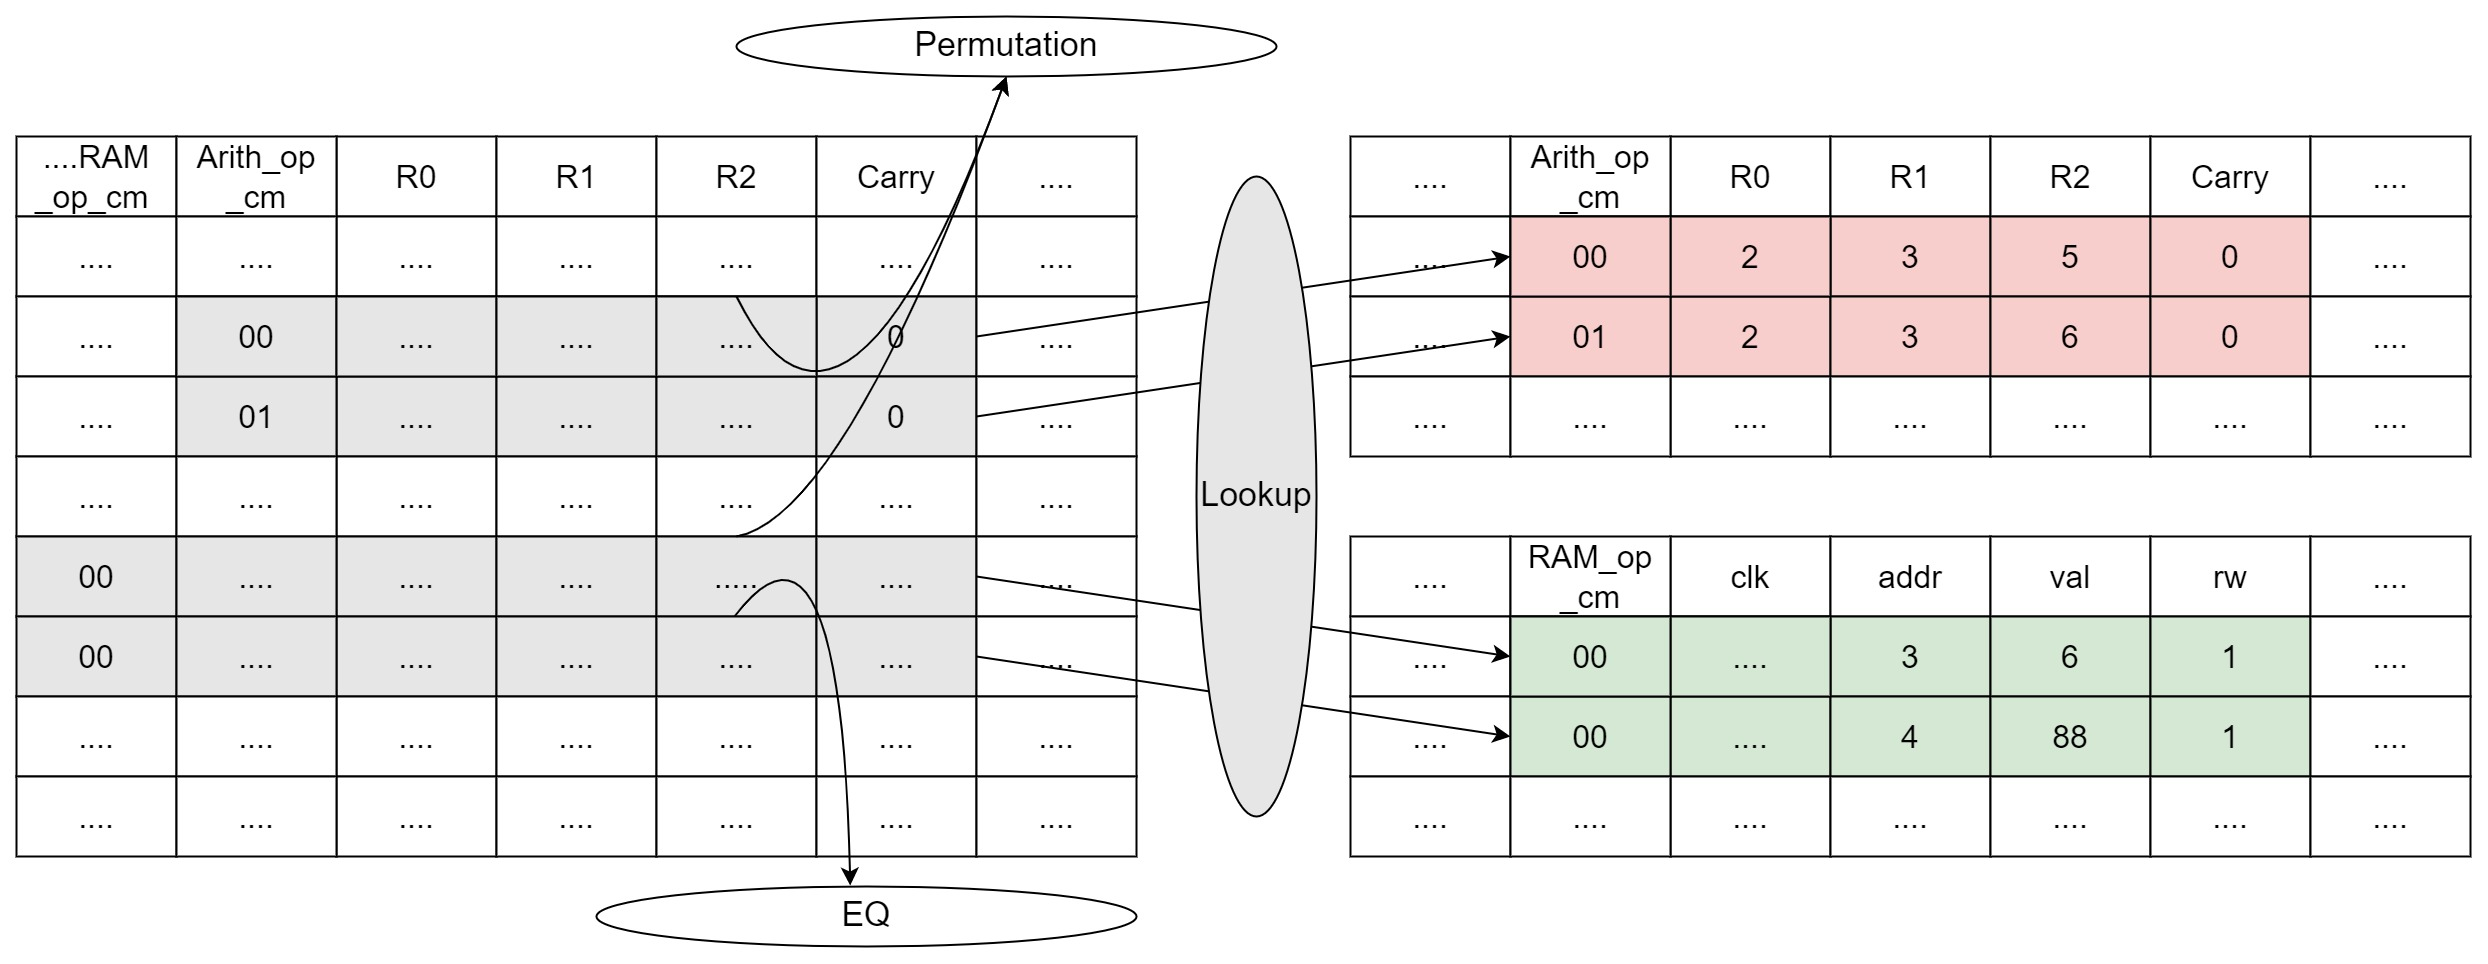
\includegraphics[width=\textwidth]{sub-sub-trace-lookup.jpg}
    \caption{Consistency between sub trace tables}
    \label{fig:sub-sub-trace-lookup}
\end{figure}
